\documentclass[12pt,letterpaper]{article}
\usepackage[latin1]{inputenc}
\usepackage[spanish]{babel}
\usepackage{amsmath}
\usepackage{amsfonts}
\usepackage{amssymb}
\usepackage{graphicx}
\usepackage[hidelinks]{hyperref}
\usepackage{color}
\graphicspath{{Imagenes/}}
\usepackage[left=2cm,right=2cm,top=2cm,bottom=2cm]{geometry}

\author{M�rquez M�rquez Amairani Ivette}
\title{EV 2.2 Explicar los arreglos y par�metros de los Amplificadores Clase A}
\date{1 de octubre de 2019}
\begin{document}
\begin{center}
\textbf{\huge {Universidad Politecnica de la Zona \\[0.5cm]Metropolitana de Guadalajara}}
\end{center}

\begin{center}

\includegraphics[width=0.65\textwidth]{UPCDLZMDG5783-logo}\\[2cm]
\end{center}
\vspace{0.1cm}
{\large\textbf{Evidencia:} 2.2 Explicar los arreglos y par�metros de los Amplificadores Clase A\\[0.2cm]\textbf{Alumna:} M�rquez M�rquez Amairani Ivette\\[0.2cm]\textbf {Profesor:} Mor�n Garabito Carlos Enrique\\[0.2cm]\textbf{Carrera:}
Ing.Mecatronica\\[0.2cm]\textbf{Grupo:}
4�B\\[0.2cm]\textbf{Fecha de entrega:}
1 de octubre del 2019\\[0.2cm]}

\vspace{10cm}
\begin{center}
\textbf{Ev 2.2 Explicar los arreglos y par�metros de los Amplificadores Clase A}
\end{center}

\vspace{0.3cm}

Un \textbf {amplificador de clase A} nos ofrece una se�al de salida igual a la de la entrada. Como se puede observar en la siguiente imagen la salida del amplificador:

\begin{figure}[hbpt]
\centering
	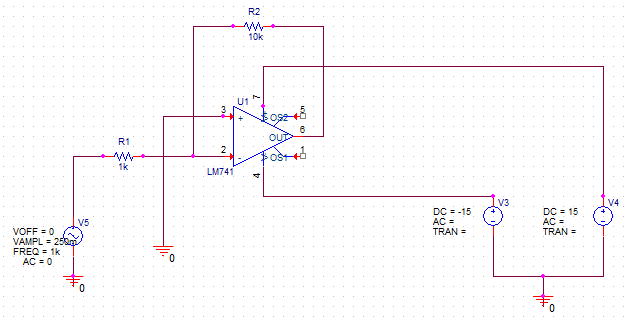
\includegraphics[width=6cm]{Imagenes/Captura_1.PNG} 
\end{figure}

\vspace{0.3cm}

La m�xima se�al de salida se puede obtener cuando el punto est�tico coincida con el centro de la recta de carga, por tanto la m�xima potencia de salida.\\
Para el amplificador de clase A se pueden presentar dos casos en cuanto a la conexi�n de la carga esto sucede cuando la potencia es externa al circuito o, esta sea la propia carga del transistor. Por lo que cualquiera de las dos se han de ver bajo el punto de vista de las rectas de carga: en el primero, son distintas para c.c y c.a y en el segundo coincide para cargas resistivas.\\
Como se observa en la siguiente imagen:

\begin{figure}[hbpt]
\centering
	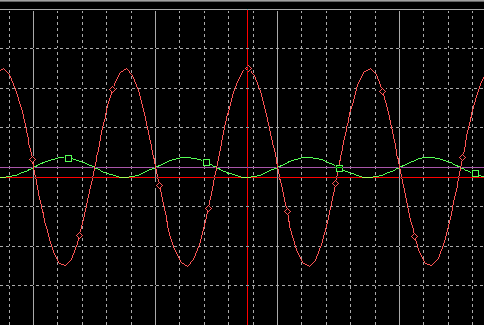
\includegraphics[width=10cm]{Imagenes/Captura_2.PNG}  
\end{figure}

\vspace{10cm}

En termino general un amplificador de potencia es aquel que, recibiendo una se�al de amplitud de tension suficiente, le aplica una elevada ganancia de corriente, capaz de gobernar cargas de baja impedancia.

\vspace{2cm}

{\large\textbf{Bibliograf�a}}\\
\begin{center}
\emph{Morales.V (03 de 2011). Amplificadores clase A y B - PDF.} Obtenido de:
\textcolor{blue}{https://electronicavm.files.wordpress.com/2011/03/amplificadores-clase-a-y-b1.pdf}\\[0.3cm]
\end{center}

\begin{center}
\emph {Lucas, J. P. (18 de Mayo de 2018). Amplificador de potencia: CLASE A (Un par de aclaraciones).} Obtenido de Electr�nica FP:\\
\textcolor{blue}{Video de youtube Amplificador de potencia: CLASE A (Un par de aclaraciones)}
\end{center}


\end{document}